% Options for packages loaded elsewhere
\PassOptionsToPackage{unicode}{hyperref}
\PassOptionsToPackage{hyphens}{url}
\PassOptionsToPackage{dvipsnames,svgnames,x11names}{xcolor}
%
\documentclass[
]{article}

\usepackage{amsmath,amssymb}
\usepackage{iftex}
\ifPDFTeX
  \usepackage[T1]{fontenc}
  \usepackage[utf8]{inputenc}
  \usepackage{textcomp} % provide euro and other symbols
\else % if luatex or xetex
  \usepackage{unicode-math}
  \defaultfontfeatures{Scale=MatchLowercase}
  \defaultfontfeatures[\rmfamily]{Ligatures=TeX,Scale=1}
\fi
\usepackage{lmodern}
\ifPDFTeX\else  
    % xetex/luatex font selection
\fi
% Use upquote if available, for straight quotes in verbatim environments
\IfFileExists{upquote.sty}{\usepackage{upquote}}{}
\IfFileExists{microtype.sty}{% use microtype if available
  \usepackage[]{microtype}
  \UseMicrotypeSet[protrusion]{basicmath} % disable protrusion for tt fonts
}{}
\makeatletter
\@ifundefined{KOMAClassName}{% if non-KOMA class
  \IfFileExists{parskip.sty}{%
    \usepackage{parskip}
  }{% else
    \setlength{\parindent}{0pt}
    \setlength{\parskip}{6pt plus 2pt minus 1pt}}
}{% if KOMA class
  \KOMAoptions{parskip=half}}
\makeatother
\usepackage{xcolor}
\usepackage[top=20mm,left=20mm,right=20mm,bottom=20mm]{geometry}
\setlength{\emergencystretch}{3em} % prevent overfull lines
\setcounter{secnumdepth}{-\maxdimen} % remove section numbering
% Make \paragraph and \subparagraph free-standing
\ifx\paragraph\undefined\else
  \let\oldparagraph\paragraph
  \renewcommand{\paragraph}[1]{\oldparagraph{#1}\mbox{}}
\fi
\ifx\subparagraph\undefined\else
  \let\oldsubparagraph\subparagraph
  \renewcommand{\subparagraph}[1]{\oldsubparagraph{#1}\mbox{}}
\fi


\providecommand{\tightlist}{%
  \setlength{\itemsep}{0pt}\setlength{\parskip}{0pt}}\usepackage{longtable,booktabs,array}
\usepackage{calc} % for calculating minipage widths
% Correct order of tables after \paragraph or \subparagraph
\usepackage{etoolbox}
\makeatletter
\patchcmd\longtable{\par}{\if@noskipsec\mbox{}\fi\par}{}{}
\makeatother
% Allow footnotes in longtable head/foot
\IfFileExists{footnotehyper.sty}{\usepackage{footnotehyper}}{\usepackage{footnote}}
\makesavenoteenv{longtable}
\usepackage{graphicx}
\makeatletter
\def\maxwidth{\ifdim\Gin@nat@width>\linewidth\linewidth\else\Gin@nat@width\fi}
\def\maxheight{\ifdim\Gin@nat@height>\textheight\textheight\else\Gin@nat@height\fi}
\makeatother
% Scale images if necessary, so that they will not overflow the page
% margins by default, and it is still possible to overwrite the defaults
% using explicit options in \includegraphics[width, height, ...]{}
\setkeys{Gin}{width=\maxwidth,height=\maxheight,keepaspectratio}
% Set default figure placement to htbp
\makeatletter
\def\fps@figure{htbp}
\makeatother
\newlength{\cslhangindent}
\setlength{\cslhangindent}{1.5em}
\newlength{\csllabelwidth}
\setlength{\csllabelwidth}{3em}
\newlength{\cslentryspacingunit} % times entry-spacing
\setlength{\cslentryspacingunit}{\parskip}
\newenvironment{CSLReferences}[2] % #1 hanging-ident, #2 entry spacing
 {% don't indent paragraphs
  \setlength{\parindent}{0pt}
  % turn on hanging indent if param 1 is 1
  \ifodd #1
  \let\oldpar\par
  \def\par{\hangindent=\cslhangindent\oldpar}
  \fi
  % set entry spacing
  \setlength{\parskip}{#2\cslentryspacingunit}
 }%
 {}
\usepackage{calc}
\newcommand{\CSLBlock}[1]{#1\hfill\break}
\newcommand{\CSLLeftMargin}[1]{\parbox[t]{\csllabelwidth}{#1}}
\newcommand{\CSLRightInline}[1]{\parbox[t]{\linewidth - \csllabelwidth}{#1}\break}
\newcommand{\CSLIndent}[1]{\hspace{\cslhangindent}#1}

\usepackage{booktabs}
\usepackage{longtable}
\usepackage{array}
\usepackage{multirow}
\usepackage{wrapfig}
\usepackage{float}
\usepackage{colortbl}
\usepackage{pdflscape}
\usepackage{tabu}
\usepackage{threeparttable}
\usepackage{threeparttablex}
\usepackage[normalem]{ulem}
\usepackage{makecell}
\usepackage{xcolor}
\usepackage{caption}
%line numbers
%\usepackage{mathpazo}
%\usepackage{rotating}
\usepackage{lineno}
\linenumbers

\usepackage[noblocks]{authblk}
\renewcommand*{\Authsep}{, }
\renewcommand*{\Authand}{, }
\renewcommand*{\Authands}{, }
\renewcommand\Affilfont{\small}
\makeatletter
\makeatother
\makeatletter
\makeatother
\makeatletter
\@ifpackageloaded{caption}{}{\usepackage{caption}}
\AtBeginDocument{%
\ifdefined\contentsname
  \renewcommand*\contentsname{Table of contents}
\else
  \newcommand\contentsname{Table of contents}
\fi
\ifdefined\listfigurename
  \renewcommand*\listfigurename{List of Figures}
\else
  \newcommand\listfigurename{List of Figures}
\fi
\ifdefined\listtablename
  \renewcommand*\listtablename{List of Tables}
\else
  \newcommand\listtablename{List of Tables}
\fi
\ifdefined\figurename
  \renewcommand*\figurename{Figure}
\else
  \newcommand\figurename{Figure}
\fi
\ifdefined\tablename
  \renewcommand*\tablename{Table}
\else
  \newcommand\tablename{Table}
\fi
}
\@ifpackageloaded{float}{}{\usepackage{float}}
\floatstyle{ruled}
\@ifundefined{c@chapter}{\newfloat{codelisting}{h}{lop}}{\newfloat{codelisting}{h}{lop}[chapter]}
\floatname{codelisting}{Listing}
\newcommand*\listoflistings{\listof{codelisting}{List of Listings}}
\makeatother
\makeatletter
\@ifpackageloaded{caption}{}{\usepackage{caption}}
\@ifpackageloaded{subcaption}{}{\usepackage{subcaption}}
\makeatother
\makeatletter
\@ifpackageloaded{tcolorbox}{}{\usepackage[skins,breakable]{tcolorbox}}
\makeatother
\makeatletter
\@ifundefined{shadecolor}{\definecolor{shadecolor}{rgb}{.97, .97, .97}}
\makeatother
\makeatletter
\makeatother
\makeatletter
\makeatother
\ifLuaTeX
  \usepackage{selnolig}  % disable illegal ligatures
\fi
\IfFileExists{bookmark.sty}{\usepackage{bookmark}}{\usepackage{hyperref}}
\IfFileExists{xurl.sty}{\usepackage{xurl}}{} % add URL line breaks if available
\urlstyle{same} % disable monospaced font for URLs
\hypersetup{
  pdftitle={Differences in COVID-19 vaccination in the province of Ontario across Health Regions and socio-economic strata},
  pdfauthor={Ariel Mundo Ortiz; Bouchra Nasri},
  colorlinks=true,
  linkcolor={blue},
  filecolor={Maroon},
  citecolor={Blue},
  urlcolor={Blue},
  pdfcreator={LaTeX via pandoc}}

\title{\textbf{Differences in COVID-19 vaccination in the province of
Ontario across Health Regions and socio-economic strata}}


\author[1,2,3]{Ariel Mundo Ortiz}
\author[1,2,3,*]{Bouchra Nasri}

\affil[1]{Centre de Recherches Mathématiques, University of Montreal,
Montréal, Canada}
\affil[2]{Department of Social and Preventive Medicine, École de Santé
Publique, University of Montreal, Montréal, Canada}
\affil[3]{Centre de recherche en santé publique, University of Montreal,
Montréal, Canada}
\affil[*]{Corresponding author, \url{bouchra.nasri@umontreal.ca}}


\date{}
\begin{document}
\maketitle
\ifdefined\Shaded\renewenvironment{Shaded}{\begin{tcolorbox}[boxrule=0pt, breakable, borderline west={3pt}{0pt}{shadecolor}, sharp corners, frame hidden, enhanced, interior hidden]}{\end{tcolorbox}}\fi

\hypertarget{abstract}{%
\section{Abstract}\label{abstract}}

The COVID-19 pandemic continues to be a worldwide public health concern.
Although vaccines against this disease were rapidly developed,
vaccination uptake has not been equal across all the segments of the
population. In particular, it has been shown that there have been
differences in vaccine uptake across different segments of the
population. However, there are also differences in vaccination across
geographical areas, which might be important to consider in the
development of future public health vaccination policies. In this study,
we examined the relationship between vaccination status (having received
the first dose of a COVID-19 vaccine), and different socio-economic and
geographical factors. Our results show that between October of 2021 and
January of 2022, individuals from underrepresented communities were
three times less likely to be vaccinated than White/Caucasian
individuals across the province of Ontario in Canada, and that in some
cases, within these groups, individuals in low-income brackets had
significantly higher odds of vaccination when compared to their peers in
high income brackets. Finally, we identified significantly lower odds of
vaccination in the Central, East and West Health Regions of Ontario
within certain underrepresented groups. This study shows that there is
an ongoing need to better understand and address differences in
vaccination uptake across diverse segments of the population of Ontario
that the pandemic has largely impacted.

\hypertarget{keywords}{%
\section*{Keywords}\label{keywords}}
\addcontentsline{toc}{section}{Keywords}

Covid-19, vaccination, survey, socio-economic factors, visible
minorities.

\hypertarget{background}{%
\section{Background}\label{background}}

As of May of 2023, there have been 765 million confirmed cases of
COVID-19 around the world, including 6.8 million
deaths\textsuperscript{\protect\hyperlink{ref-WHO-Covid}{1}}. Although
this disease is no longer categorized as a global health emergency by
the World Health Organization
(WHO)\textsuperscript{\protect\hyperlink{ref-rigby2023}{2}}, there is
ongoing concern due to continued transmission, the possibility of surges
in cases and deaths due to new virus
variants\textsuperscript{\protect\hyperlink{ref-un2023}{3}}, and ongoing
issues in health systems around the world that could be exploited by a
novel virus or another public health emergency in the
future\textsuperscript{\protect\hyperlink{ref-mackey2021}{4}}.

In particular, the pandemic showed multiple challenges with regard to
vaccination. The rapid development of vaccines against COVID-19
initially brought the hope of a rapid end to the pandemic as vaccination
campaigns in certain parts of the world started as early as December of
2020\textsuperscript{\protect\hyperlink{ref-thelancet2021}{5}--\protect\hyperlink{ref-tanne2020}{8}}.
Although it has been estimated that so far COVID-19 vaccines have been
able to prevent millions of deaths
worldwide\textsuperscript{\protect\hyperlink{ref-watson2022}{9}}, their
implementation has faced multiple challenges across the world. These
challenges included the rapid emergence of new virus
variants\textsuperscript{\protect\hyperlink{ref-li2021}{10}}, the waning
of vaccine
protection\textsuperscript{\protect\hyperlink{ref-dolgin2021}{11}},
inequality in vaccine access between high-income and low-income
countries\textsuperscript{\protect\hyperlink{ref-gerretsen2021}{12},\protect\hyperlink{ref-tamey2022}{13}},
vaccine
hesitancy\textsuperscript{\protect\hyperlink{ref-nafilyan2021}{14}}, and
differences in vaccine uptake across the
population\textsuperscript{\protect\hyperlink{ref-willis2021}{15},\protect\hyperlink{ref-skirrow2022}{16}}.
In particular, it is well established that lower vaccination uptake has
been observed in individuals within certain underrepresented groups
(e.g., Black, Asian, or Indigenous) as well as individuals with
socio-economic
disadvantages\textsuperscript{\protect\hyperlink{ref-willis2021}{15}--\protect\hyperlink{ref-hussain2022}{21}}.

Reasons given for this inequality in vaccination uptake have included
medical mistrust due to systemic medical
racism\textsuperscript{\protect\hyperlink{ref-stoler2021}{17},\protect\hyperlink{ref-mosby2021}{22}},
mistrust in
vaccines\textsuperscript{\protect\hyperlink{ref-willis2021}{15}}, and
the existence of health misinformation and
disinformation\textsuperscript{\protect\hyperlink{ref-mosby2021}{22}--\protect\hyperlink{ref-freeman2020}{24}}.
However, it is important also to consider that vaccination uptake can be
influenced by geographical (spatial) factors. In this regard,
differences in COVID-19 vaccination rates have been associated with
varied regional attitudes towards
vaccination\textsuperscript{\protect\hyperlink{ref-malik2020}{25}}, lack
of vaccine access in areas where underrepresented groups
reside\textsuperscript{\protect\hyperlink{ref-bogoch2022}{7}}, as well
as an absence of prioritization of areas inhabited by vulnerable
groups\textsuperscript{\protect\hyperlink{ref-nguyen2021}{26}}. Other
studies have also shown heterogeneity in vaccine uptake within small
governmental administrative units such as
counties\textsuperscript{\protect\hyperlink{ref-mollalo2021}{27}--\protect\hyperlink{ref-bhuiyan2022}{30}},
indicating that accounting for geographical differences in vaccination
can help predict patterns of booster
uptake\textsuperscript{\protect\hyperlink{ref-wood2022}{31}}. However,
there is a limited amount of studies that have analyzed geographical
differences in vaccination in Canada. Existing studies in this area have
focused on differences within certain cities, such as
Toronto\textsuperscript{\protect\hyperlink{ref-choi2021}{32}}, or
Montréal\textsuperscript{\protect\hyperlink{ref-mckinnon2021}{33}}), or
have explored differences between
provinces\textsuperscript{\protect\hyperlink{ref-guay2022}{19}}, but to
our knowledge, there are no studies that analyze differences in
vaccination uptake at the intra-provincial level. Such need is specially
important in the context of Canada's pandemic response goals, which have
been to minimize serious illness and deaths while minimizing societal
disruption\textsuperscript{\protect\hyperlink{ref-naci2023}{34}}.
Analyzing differences in vaccination uptake within the provinces can aid
to identify inequalities that might exist and that need to be addressed
before the advent of another pandemic.

This need is especially important in the case of Ontario, the most
populated province of Canada, and which as has a complex healthcare
system. Between 2007 and 2019, Ontario managed healthcare access to its
inhabitants using 14 intra-provincial divisions called the Local Health
Integration Networks (LHINs), which aimed to provide an integrated
health system. However, this approach was complex, bureaucratic,
resulting in excessive expenditures, disparities in mortality rates, the
deterioration of certain performance indicators (such as wait times and
hospital readmissions), fragmented electronic health systems, and
inequities in health services
access\textsuperscript{\protect\hyperlink{ref-tsasis2012}{35}--\protect\hyperlink{ref-lysyk2016}{39}}.
With the intent of better organizing and delivering care, in late 2019
the provincial government eliminated the LHINs and incorporated the
areas covered by them into six larger Health Regions (North East, North
West, Central, Toronto, West, and East), which are managed by a new
government agency, Ontario Health
(OH)\textsuperscript{\protect\hyperlink{ref-dong2022}{37}}.

On the other hand, public health in Ontario is administered by Public
Health Ontario (PHO), a government agency established in late 2007 and
that is currently composed of 34 Public Health Units (PHUs) that cover
the entire geography of the province. Although PHUS were commissioned
with leading the distribution of the COVID-19 vaccine within their
respective
areas\textsuperscript{\protect\hyperlink{ref-rotenberg2021}{40}}, the
vaccine rollout occurred with significant interaction between PHO and
OH; in many instances both agencies had to work together to organize
vaccination clinics, with personnel associated with OH also being
actively involved when demand exceeded the capacity of PHO personnel,
especially in rural
areas\textsuperscript{\protect\hyperlink{ref-ashcroft2023}{41}}. Indeed,
based on the experience of COVID-19, there is an ongoing debate on how
OH and PHO will interact in the future, and the challenges that this
will entail for the healthcare system of the
province\textsuperscript{\protect\hyperlink{ref-dion2022}{42}}.

Therefore, considering the relatively recent adoption of the Health
Region model and its alignment with the onset of the COVID-19 pandemic,
there is an ongoing need to analyze the existence of geographical
disparities in vaccination uptake within the Health Regions and identify
the socio-demographic groups that might be affected, as this can serve
as an indirect assessment of the state of the implementation of the new
model while helping identify ongoing challenges that decision-makers
might need to address to ensure the long-term success of this model and
its interaction with PHO, which is specially important considering that
previous research has highlighted disparities in the level of activity
of each Health
Region\textsuperscript{\protect\hyperlink{ref-sethuram2023}{43}}.

Therefore, in this study we hypothesized that there were differences in
COVID-19 vaccination rates between the Health Regions between October
2021 and January of 2022. To understand and contextualize these
differences, we by included socio-economic factors in our analysis,
aiming to identify in which demographic groups were particularly
impacted, in order to provide an assessment of the current state of
healthcare access in Ontario.

\hypertarget{methods}{%
\section{Methods}\label{methods}}

\hypertarget{sec-data}{%
\subsection{Data and Methods}\label{sec-data}}

We used data from the \emph{Survey of COVID-19 related Behaviours and
Attitudes}, a repeated cross sectional survey focused on the Canadian
province of Ontario that was commissioned by the Fields Institute for
Research in Mathematical Sciences and the Mathematical Modelling of
COVID-19 Task Force under ethical guidance from the University of
Toronto (under Research Ethics Board approval \#40999), and which ran
between September 30th, 2021 and January 17th,2022.

Briefly, the survey was deployed using random domain intercept
technology, a methodology where internet users whose device meta-data
indicated their presence in the province of Ontario had a random chance
of being redirected to the survey after they had clicked on a registered
but commercially inactive web link, or typed in a web address for a site
that was dormant but that was temporarily managed by the company that
administered the survey (RIWI
Corp)\textsuperscript{\protect\hyperlink{ref-sargent2022}{44}}. Users
then decided whether to anonymously participate in the survey, and those
that participated were able to exit the survey at any time. After the
survey closed, regardless if it was complete or incomplete, access was
denied to any further users with the same internet protocol address
(IP), effectively allowing each user only one opportunity to participate
in the survey. Users who indicated they were under the age of 16 were
exited from the survey without creating a record. Finally, the personal
identifier information from each user that participated in the survey
was automatically scrubbed and replaced by a unique ID.

Survey users entered their socio-economic information (age, income, and
racial/ethnic group), and asked information on vaccination status by
using the question ``Have you received the first dose of the COVID
vaccine?'', with possible answers ``yes'' and ``no''
(Table~\ref{tbl-descriptive-stats}). Of notice, because the
racial/ethnic categories of the survey did not match exactly the
categories from the 2016 Census, we used a combination of sources to
re-group certain categories in order to obtain estimates that could be
used to correct the data. Further details can be found in the Appendix.

Additionally, the survey automatically collected the geographical
location of the respondent (using the nearest municipality, as shown in
Figure~\ref{fig-map}), and the date of access to the survey. The
original dataset contained 39,029 observations with a response rate of
16.25\% (observations where users had complete answers), due to the
survey design that allowed respondents to exit at any time and deployed
the questions randomly. We selected these observations with complete
answers (6,343 observations) for our analysis. Later, we matched the
city of each observation with its corresponding LHIN and Health Region,
and removed observations from areas with low representation (254
observations corresponding to the North West and North East Health
Regions). After all the preliminary analyses, the total number of
observations used for analysis was 6,236 and included the East, Central,
Toronto, and West Health Regions covering between October 1st,2021 and
January 17, 2022. The original dataset, clean dataset, and details on
the data cleaning process are described in detail in the
\href{https://github.com/aimundo/Fields_COVID-19/}{GitHub repository}
for this paper.

\begin{figure}

{\centering 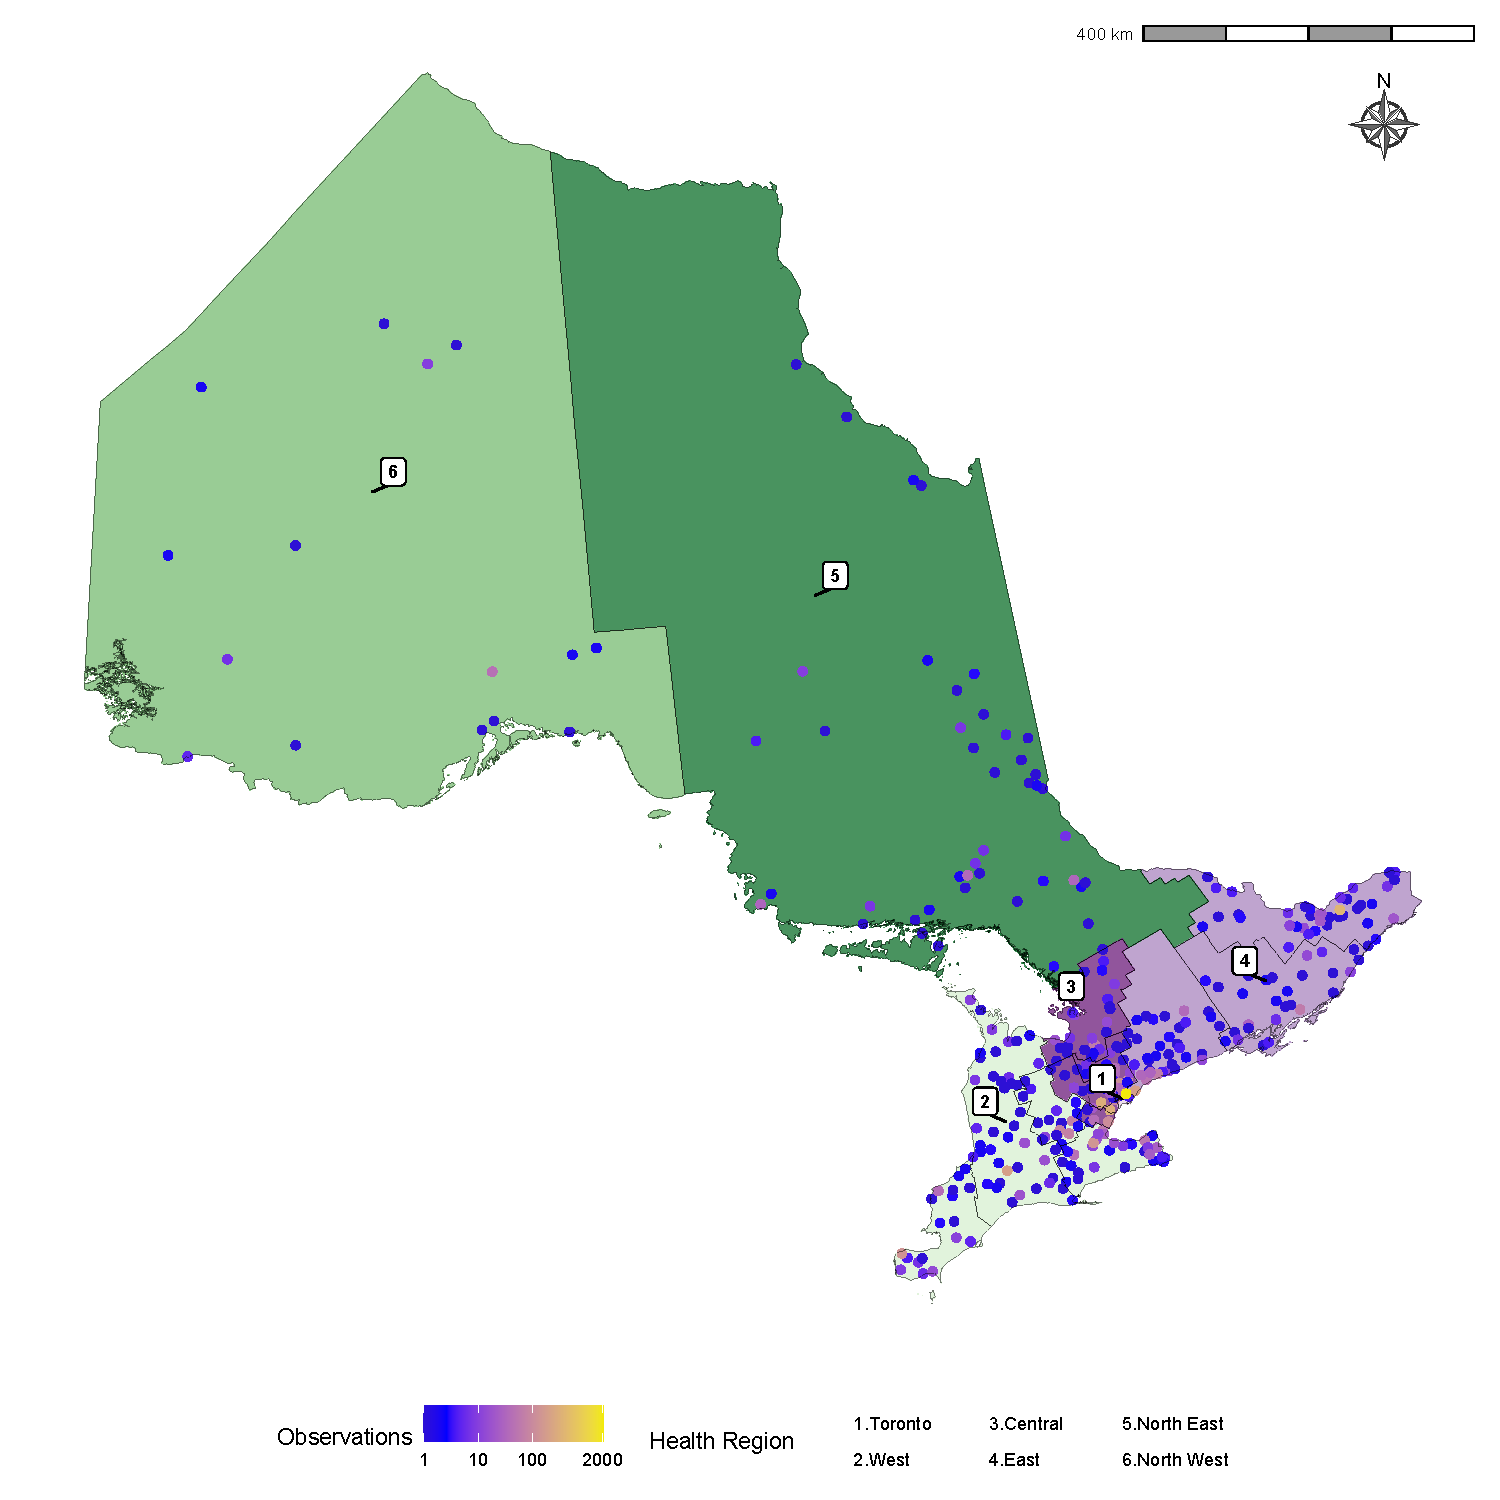
\includegraphics[width=1\textwidth,height=1\textheight]{../data/map_data/map_June_01.pdf}

}

\caption{\label{fig-map}Geographic representation of the data collected
by the \emph{Survey of COVID-19 related Behaviours and Attitudes},
collected by the Fields Institute in Ontario. Municipalities from where
survey participants provided answers appear as points, color indicates
number of observation obtained from each city. The Health six Regions
are color-coded and labelled sequentially. Internal boundaries within
certain Health Regions indicate areas previously covered by the Local
Integrated Health Networks (LHINs).}

\end{figure}

\hypertarget{statistical-analyses}{%
\subsection{Statistical analyses}\label{statistical-analyses}}

We used a logistic regression model to examine the impact of the Health
Regions in vaccination rates while considering the socio-economic
factors and months covered by the survey
(Table~\ref{tbl-descriptive-stats}) and certain interactions (Race and
Health Region and Race and income), as previous studies have shown that
socio-economic factors and their interactions are significant predictors
of intent of vaccination and vaccination
status\textsuperscript{\protect\hyperlink{ref-nguyen2022}{45}--\protect\hyperlink{ref-cnat2022a}{47}}.
Because we identified differences in representativity between the survey
data and the estimates from the 2016 Census for the variables considered
in the analysis, and used used an iterative proportional fitting
procedure
(\emph{raking})\textsuperscript{\protect\hyperlink{ref-deming1940}{48}}
to correct the data using data from the Census and Health Region
population totals; and fitted the regression model to the uncorrected
and corrected data. Details regarding the correction can be found in the
Appendix. All analyses were conducted in R 4.2.2 using the packages
\texttt{survey}\textsuperscript{\protect\hyperlink{ref-lumley2011}{49}},\texttt{tidyverse}\textsuperscript{\protect\hyperlink{ref-wickham2019}{50}},
\texttt{quarto}\textsuperscript{\protect\hyperlink{ref-quarto}{51}},
\texttt{modelsummary}\textsuperscript{\protect\hyperlink{ref-modelsummary}{52}},
and
\texttt{gtsummary}\textsuperscript{\protect\hyperlink{ref-gtsummary}{53}}.

\hypertarget{results}{%
\section{Results}\label{results}}

\hypertarget{sample-characteristics}{%
\subsection{Sample Characteristics}\label{sample-characteristics}}

Table~\ref{tbl-descriptive-stats} shows the characteristics of the data
from the Fields COVID-19 survey used for analysis. The sample contained
6,236 observations, from which 24.8\% (1,547) corresponded to
individuals that reported not having initiated a COVID-19 vaccine
primary series (in other words, not having received the first dose of
the vaccine). The rate for the first dose of the vaccine ranged between
71-79\% across all household income brackets, age groups, Health
Regions, and the months considered in the survey. However, the highest
rate for the uptake of the first dose of the vaccine were reported by
individuals in the highest income bracket (79\%), those between 16 and
34 years of age (77\%), individuals that lived in the East Health Region
(77\%), and during January of 2022 (78\%). Between racial/ethnic groups,
White/Caucasian individuals reported the highest uptake of the first
dose of the vaccine (84\%), against values that ranged between 63 and
66\% in the case of Arab/Middle Eastern, Black, Indigenous, Latin
American individuals, and those that belonged to the ``other'' racial
group category (which included Southeast Asian, Filipino, West Asian,
and minorities not identified elsewhere percentages ).

\hypertarget{tbl-descriptive-stats}{}
\setlength{\LTpost}{0mm}
\begin{longtable}{lccc}
\caption{\label{tbl-descriptive-stats}Descriptive Statistics of the Fields COVID-19 Survey (by Vaccination
Status) }\tabularnewline

\toprule
\textbf{Variable} & \textbf{no}, N = 1,547\textsuperscript{\textit{1}} & \textbf{yes}, N = 4,689\textsuperscript{\textit{1}} & \textbf{p-value}\textsuperscript{\textit{2}} \\ 
\midrule
Income (CAD) &  &  & <0.001 \\ 
    60000 and above & 542 (21\%) & 1,996 (79\%) &  \\ 
    25000-59999 & 347 (25\%) & 1,046 (75\%) &  \\ 
    under 25000 & 658 (29\%) & 1,647 (71\%) &  \\ 
Age Group &  &  & 0.002 \\ 
    16-34 & 645 (23\%) & 2,117 (77\%) &  \\ 
    35-54 & 411 (24\%) & 1,305 (76\%) &  \\ 
    55 and over & 491 (28\%) & 1,267 (72\%) &  \\ 
Health Region &  &  & 0.3 \\ 
    Toronto & 593 (26\%) & 1,709 (74\%) &  \\ 
    Central & 372 (26\%) & 1,083 (74\%) &  \\ 
    East & 236 (23\%) & 783 (77\%) &  \\ 
    West & 346 (24\%) & 1,114 (76\%) &  \\ 
Month &  &  & <0.001 \\ 
    October & 469 (27\%) & 1,263 (73\%) &  \\ 
    November & 376 (28\%) & 980 (72\%) &  \\ 
    December & 181 (24\%) & 565 (76\%) &  \\ 
    January & 521 (22\%) & 1,881 (78\%) &  \\ 
Race &  &  & <0.001 \\ 
    White/Caucasian & 354 (16\%) & 1,871 (84\%) &  \\ 
    Arab/Middle Eastern & 111 (34\%) & 220 (66\%) &  \\ 
    Black & 159 (34\%) & 303 (66\%) &  \\ 
    East Asian/Pacific Islander & 94 (19\%) & 404 (81\%) &  \\ 
    Indigenous & 112 (37\%) & 194 (63\%) &  \\ 
    Latin American & 99 (34\%) & 195 (66\%) &  \\ 
    Mixed & 177 (30\%) & 411 (70\%) &  \\ 
    Other\textsuperscript{\textit{3}} & 315 (34\%) & 606 (66\%) &  \\ 
    South Asian & 126 (21\%) & 485 (79\%) &  \\ 
\bottomrule
\end{longtable}
\begin{minipage}{\linewidth}
\textsuperscript{\textit{1}}n (\%)\\
\textsuperscript{\textit{2}}Pearson's Chi-squared test\\
\textsuperscript{\textit{3}}This category included Southeast Asian, Filipino, and West Asian individuals,
and minorities not identified elsewhere according to the 2016 Census.\\
\end{minipage}

\hypertarget{multivariate-regression}{%
\subsection{Multivariate Regression}\label{multivariate-regression}}

Figure~\ref{fig-models} presents the estimates (as odd ratios) from the
logistic regression models for vaccination status using the
socio-demographic factors collected by the survey, and their
interactions. Generally speaking, lower odds of vaccination were
identified in both cases in individuals characterized by a low household
income, or that identified as part of underrepresented groups. However,
the magnitude of the estimates differed between the uncorrected and
corrected models and more importantly, there were differences in the
statistical significance of certain estimates before and after the
correction. Specifically, the uncorrected model showed significant
differences in vaccination odds between the age groups considered, the
East Health Region, Latin American individuals with a household income
under CAD 25,000, and Indigenous individuals living in the Central
Health Region (Figure~\ref{fig-models},B) but these were deemed non
statistically significant after the correction.

\begin{figure}

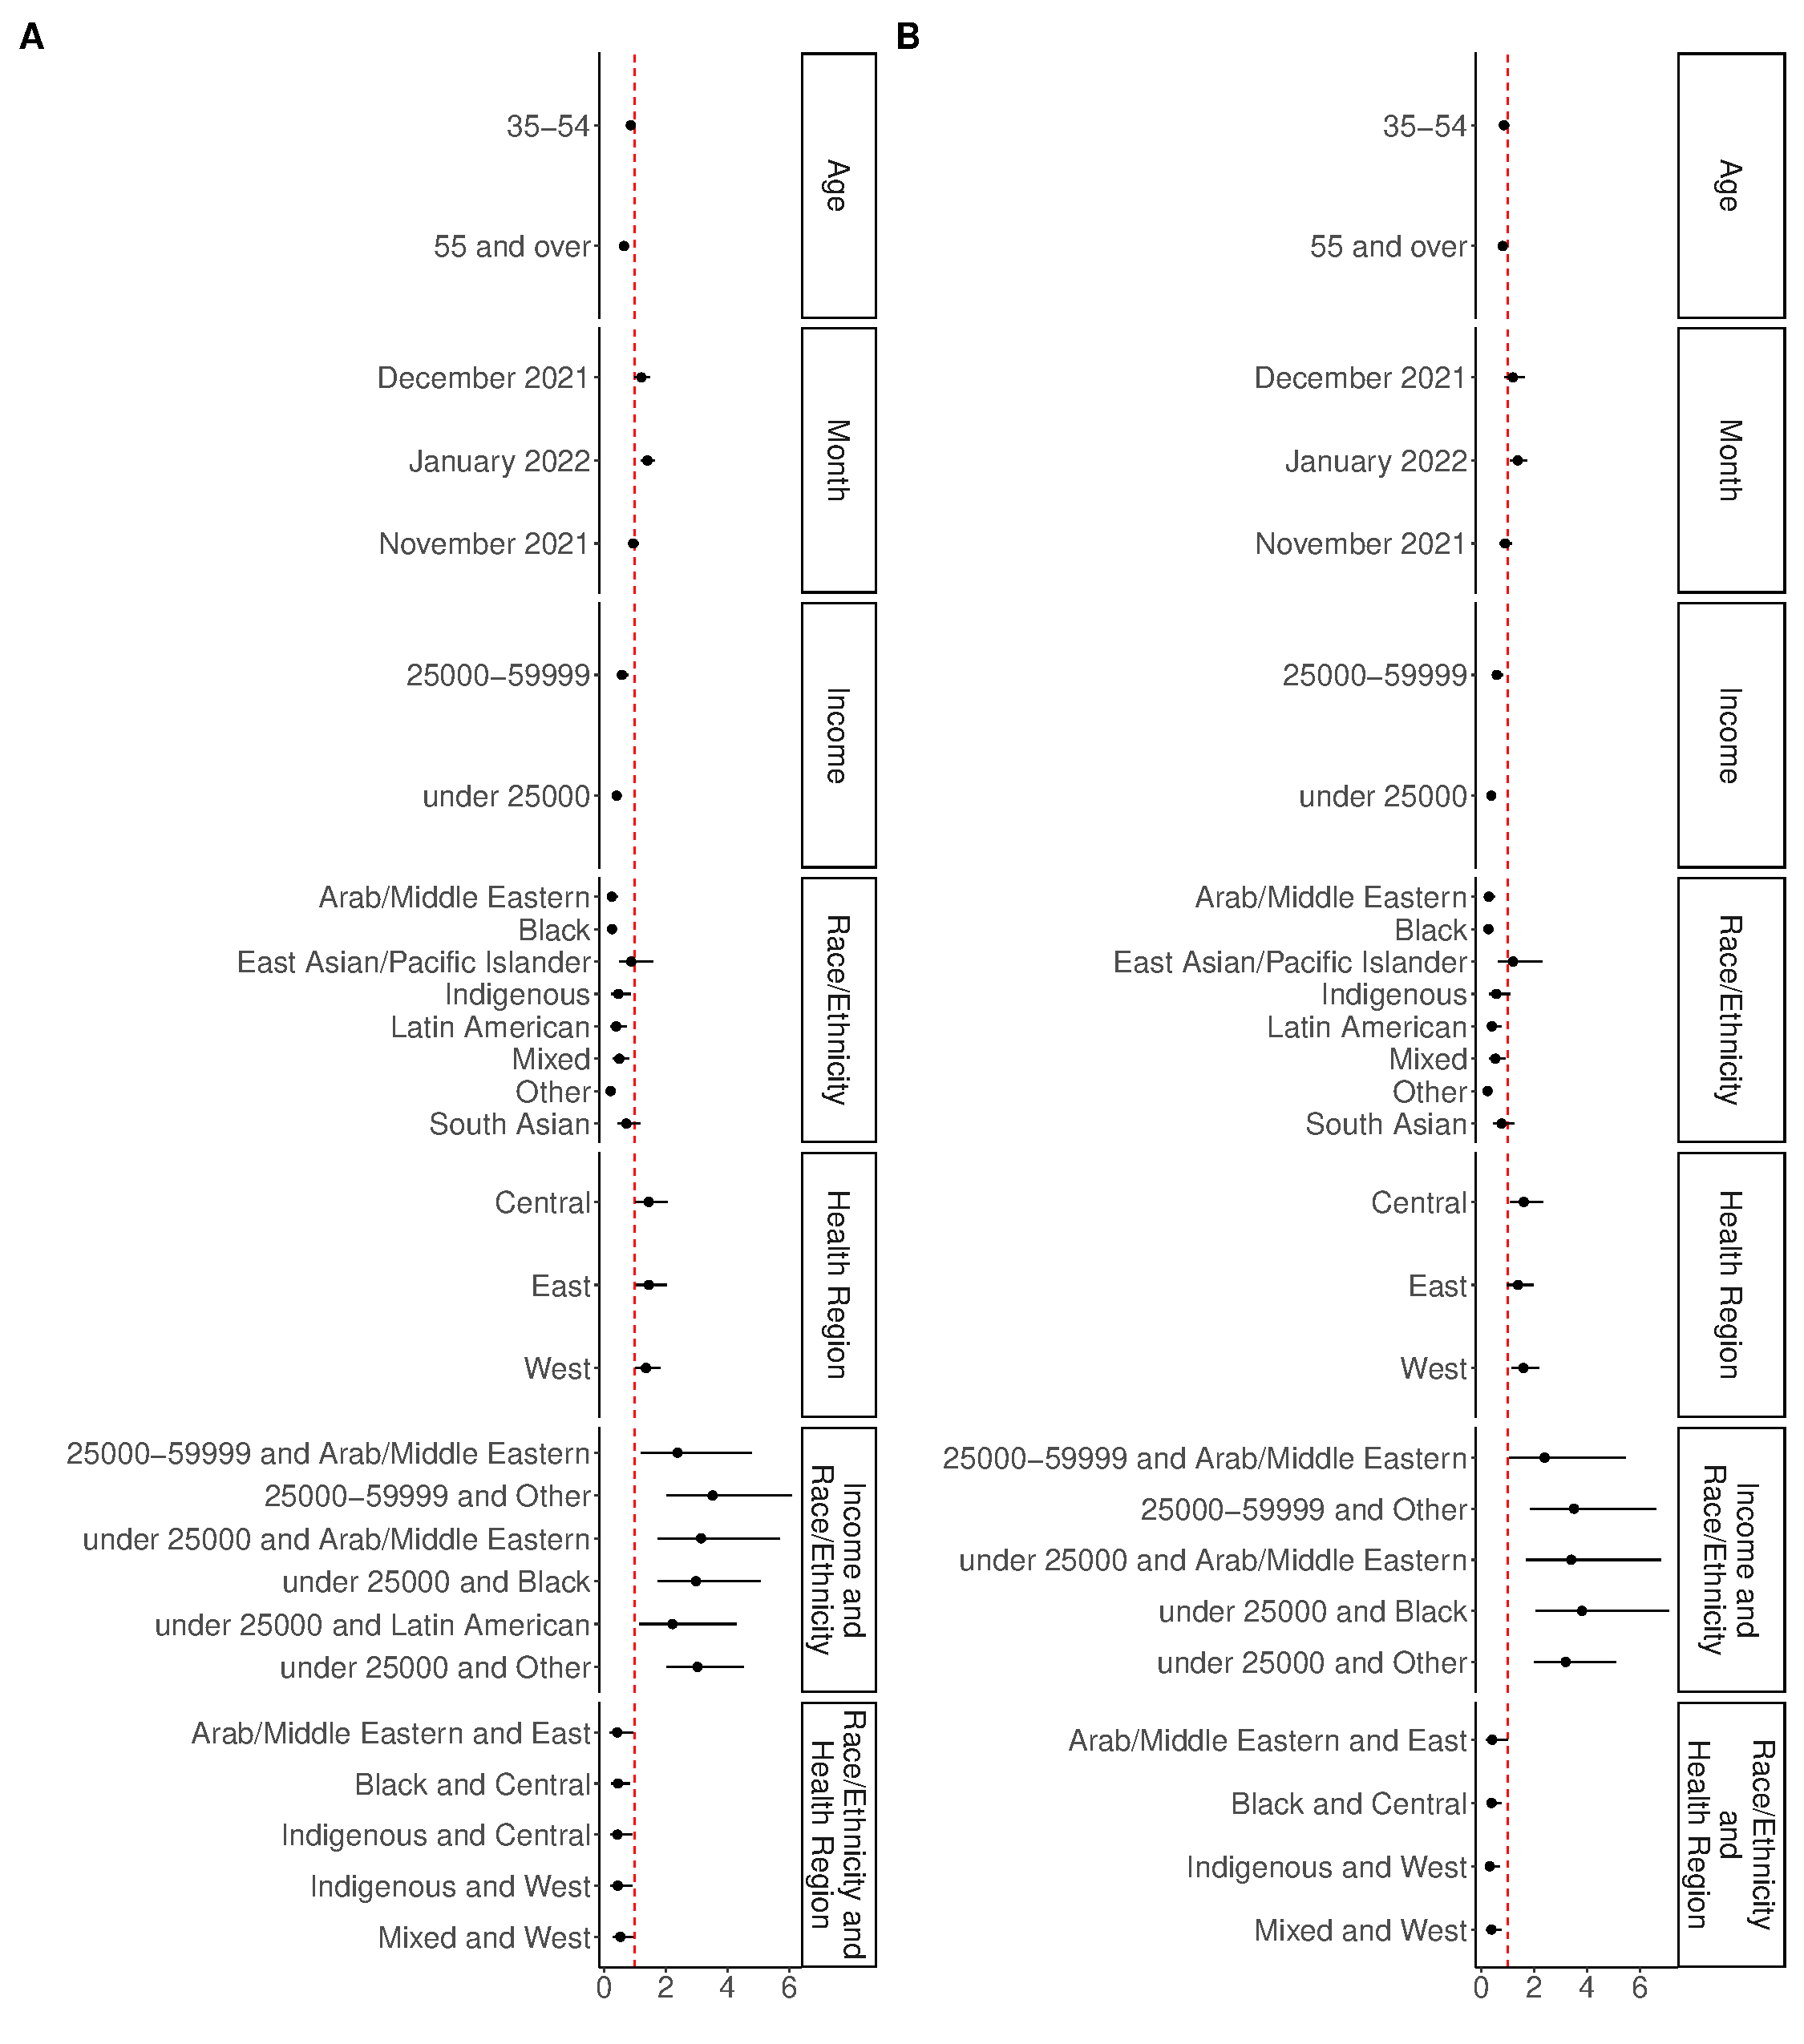
\includegraphics{main_files/figure-pdf/fig-models-1.pdf} \hfill{}

\caption{\label{fig-models}Coefficient estimates and confidence
intervals for the uncorrected model. Only statistically significant
interaction terms are shown. Full interaction terms can be found in
Supplementary Figures A-3 and A-4.}

\end{figure}

However, significantly lower odds of vaccination were identified in the
corrected model for those with a household income under CAD 25,000
(OR=0.37, CI={[}0.27,0.51{]}) and those with an income between CAD
25,000 and 59,999 (OR=0.58, CI={[}0.42,0.81{]}). Additionally,
individuals who identified as Arab/Middle Eastern, Black, Latin
American, of mixed background, or that belonged to other racial groups
(a category that included Southeast Asian, Filipino, West Asian, and
minorities not identified elsewhere), had significantly lower odds of
vaccination than those in the White/Caucasian group (ORs and CIs=0.28
{[}0.16,0.51{]}, 0.27 {[}0.16,0.45{]}, 0.40 {[}0.21,0.76{]}, 0.53
{[}0.30,0.92{]}, 0.23 {[}0.15,0.36{]}). Additionally, individuals that
reported living in the Central and West Health Regions had higher odds
of vaccination than those in the Health Region of Toronto (ORs and
CIs=1.61 {[}1.10,2.34{]}, and 1.59 {[}1.16,2.19{]}, respectively).

Interestingly, individuals in underrepresented groups with a household
income below CAD 25,000 had higher odds of vaccination (when compared to
those with a household income above CAD 60,000). This held true in the
case of Arab/Middle Eastern individuals (OR=34, CI={[}1.70,6.79{]}),
Black individuals (OR=3.81, CI={[}2.05, 7.09{]}), and those in other
racial or ethnic groups (OR=3.19, CI={[}2.00,5.09{]}). Additionally,
individuals with an income between CAD 25,000 and 59,999 in the
Arab/Middle Eastern and other racial or ethnic groups also had higher
odds of vaccination than their high-income peers (ORs and CIs=6.96
{[}2.67,18.16{]}, and 3.5 {[}1.85,6.62{]}).

Finally, the place of habitation affected the odds of vaccination for
certain underrepresented groups, as significantly lower odds of
vaccination were identified for the interaction between Health Region
and race in the case of Black individuals in the Central Health Region
(OR=0.39, CI={[}0.2,0.75{]}), Arab/Middle Eastern individuals in the
East Health Region (OR=0.41 {[}0.17, 0.98{]}), and in the Indigenous and
mixed groups in the West Health Region (ORs and CIs={[}0.31 {[}0.14,
0.7{]} and 0.38 {[}0.19, 0.76{]}, respectively).

\hypertarget{discussion}{%
\section{Discussion}\label{discussion}}

The COVID-19 pandemic has presented many significant challenges to the
healthcare systems of the Canadian
provinces\textsuperscript{\protect\hyperlink{ref-alami2021}{54}}. In the
case of Ontario, the recent adoption of the Health Region model at the
onset of the pandemic signified an additional level of complexity
because although PHO (through the 34 Public Health Units of the
province) was the lead in vaccine distribution, in reality the vaccine
rollout required active collaboration between PHO and OH in multiple
instances\textsuperscript{\protect\hyperlink{ref-ashcroft2023}{41}}.

In this study, we hypothesized that there were differences in the uptake
of the first dose of the COVID-19 vaccine between individuals living in
the different Health Regions of Ontario during late 2021 and early 2022.
Using the Health Regions as the base of our analysis was advantageous,
as these new Health Regions match closely the geographical boundaries of
the Health Regions that have been historically used to group Public
Health Units in the
province\textsuperscript{\protect\hyperlink{ref-bolotin2018}{55},\protect\hyperlink{ref-ohesi}{56}},
thus providing information with relevance at both the public health and
healthcare system level. Therefore, this analysis could provide an
overall assessment of intra-provincial disparities that might need to be
addressed moving forward by decision-makers, in order to ensure that in
the future, and specially in the event of a future public health
emergency, OH and PHO will able to collaboratively work in an efficient
way and thus ensure that the population of the province benefits in the
long term of the newly implemented Health Region model.

Our results show that indeed, there were differences in the uptake of
the first dose of the vaccine across Ontario in certain
socio-demographic groups. Specifically, those who identified as
Arab/Middle Eastern, Black, Latin American, having mixed racial or
ethnic background, or that belonged to other groups not explicitly
included in the survey (Southeast Asian, Filipino, West Asian, and
minority groups not identified elsewhere) had vaccination odds that were
between a third and a half of that of individuals that identified as
White or Caucasian (Figure~\ref{fig-models}). These results are
consistent with previous studies that have shown lower vaccination rates
in individuals with the same socio-demographic
characteristics\textsuperscript{\protect\hyperlink{ref-guay2022}{19}--\protect\hyperlink{ref-hussain2022}{21},\protect\hyperlink{ref-carter2022}{57}}.

Lower vaccine uptake in the socio-demographic groups indicated above may
be influenced in part, by vaccine hesitancy and refusal, which have been
associated in underrepresented Canadian individuals with concerns on
vaccine safety, effectiveness, and experiences of racial discrimination
in health
settings\textsuperscript{\protect\hyperlink{ref-cnat2022a}{47},\protect\hyperlink{ref-basta2022}{58}--\protect\hyperlink{ref-cnat2023}{60}}.
However, it has been shown that structural barriers also play an
important role in vaccination uptake. In the case of underrepresented
individuals, such barriers include complex scheduling systems, language
barriers, lack of adequate public transportation, and lack of accessible
vaccination
sites\textsuperscript{\protect\hyperlink{ref-njoku2021}{61}}. In this
regard, it is interesting to note that vaccination venues were scarce in
low socio-economic areas that had the highest burden of COVID-19 in
Toronto and other regions of Ontario around the time covered by the
survey\textsuperscript{\protect\hyperlink{ref-bogoch2022}{7},\protect\hyperlink{ref-iveniuk2021}{62}},
and that pharmacies in the Peel region (an area identified as a
``hotspot'' with high numbers of essential workers and multigenerational
households) could not keep up with vaccine
demand\textsuperscript{\protect\hyperlink{ref-gill2022}{63}}. This
suggests that the observed differences are associated with disparities
in vaccine access that were present during the period covered by the
survey.

Interestingly, whereas overall self-reported vaccination rates were
found to be statistically significantly lower in various
underrepresented groups when compared to White/Caucasian individuals,
the change in odds of vaccination within certain racial groups and
income strata was actually positive, in contrast to the White/Caucasian
group, where vaccination odds decreased in income brackets below CAD
60,000 (Supplementary Figure A-5). Specifically, individuals in low
income brackets that belonged to Arab/Middle Eastern, Black, or other
minority groups had higher odds of vaccination that their peers with an
income above 60,000 CAD.

This result likely reflects in part the fact that individuals in
underrepresented groups tend to perform occupations that have been
deemed as ``essential'' in the context of the
pandemic\textsuperscript{\protect\hyperlink{ref-hawkins2020}{64},\protect\hyperlink{ref-ct2021}{65}},
which include workers in the areas of grocery stores, gas stations,
warehouses, distribution, and manufacturing, all being occupations for
which an income within the significant brackets identified in the
analysis is to be expected. From one side, individuals in essential
occupations in the province experienced higher rates of morbidity and
mortality during the first year of the
pandemic\textsuperscript{\protect\hyperlink{ref-rao2021}{66}}, but later
on, they had priority for COVID-19
vaccination\textsuperscript{\protect\hyperlink{ref-mishra2021}{67}}.
Additionally, it is known that vaccination uptake in these individuals
was encouraged by vaccination staff in certain parts of the
province\textsuperscript{\protect\hyperlink{ref-gill2022}{63}}. These
facts, combined with evidence of increased trends in vaccination in this
group
elsewhere\textsuperscript{\protect\hyperlink{ref-nguyen2021b}{68}},
suggest that in Ontario, the type of occupation of individuals in
underrepresented groups (which might have also affected their decision
to get a vaccine based on their knowledge of increased risk), played an
important role in the higher the odds of vaccination observed in these
individuals.

However, the results also indicate that the place of habitation affected
the odds of vaccination for certain underrepresented groups (interaction
term of Health Region and Race, Figure~\ref{fig-models},B).
Specifically, this held true in the case of individuals identifying as
Indigenous or with mixed racial background in the West Health Region,
Black individuals in the Central Health Region, and Arab/Middle Eastern
individuals in the East Health Region Figure~\ref{fig-models}. For these
individuals, vaccination odds were lower when compared to the Toronto
Health Region (Supplementary Figure A-6). We indicate next some
contributing factors that might help provide context to these results.

First, in this case it is useful to analyze the data considering the
LHINs in each Health Region, because most studies in the literature
focused on Ontario use the LHINs as the base of their analyses. The West
Health Region covers the area previously occupied by the Hamilton
Niagara Haldimand Brant, South West, and Waterloo Wellington LHINs,
whereas the East Health Region covers the area of the former Champlain
and Central East LHINs. Previous research has identified health
disparities in these (mostly rural) regions, such as unequal
distribution of primary care providers, increased mortality, and low
pharmacist
availability\textsuperscript{\protect\hyperlink{ref-shah2019}{69}--\protect\hyperlink{ref-timony2022}{71}}.

Furthermore, there is an ongoing challenge for the health system of the
province with regard to personalized healthcare for marginalized
individuals. For example, the West Health Region has only two Aboriginal
Health Access Centres (community-led primary healthcare organizations
focused on First Nations, Métis, and Inuit communities) to provide care
to an estimated 100,000 Indigenous individuals living in the
area\textsuperscript{\protect\hyperlink{ref-ontariohealth}{72}}. Lack of
access to personalized healthcare affects individuals that may mistrust
the traditional healthcare system due to systemic racism or oppression,
which is known to be the case for Indigenous and Black individuals in
Canada, as these rationales have been associated with observed lower
vaccination rates among these
groups\textsuperscript{\protect\hyperlink{ref-smylie2022}{73},\protect\hyperlink{ref-eissa2021}{74}}.
Taken together, this suggests that healthcare disparities specific to
these underrepresented groups in certain parts of the province impacted
vaccination uptake, and highlights the need of investments in the Health
Regions focused on resources, infrastructure, and specially personnel
that can deliver personalized care to marginalized communities, as it
has been shown that such efforts have improved trust in vaccination in
underrepresented groups
elsewhere\textsuperscript{\protect\hyperlink{ref-schafferderoo2020}{75}}.

There are some limitations to the present study. First, the data
collection design, which allowed respondents to withdraw from the survey
at any point, and that deployed the questions in a random manner
resulted in an elevated number of missing observations without a
definite pattern and complicated the implementation of sensitivity
analyses. Therefore, we focused on entries that had complete answers,
and corrected the data using population-wide information from the
Census. However, more granular corrections would be needed to obtain
more accurate estimates: For example, our analysis identified higher
odds of vaccination in the Central and West Health Regions, but in this
case these differences are likely to be driven by the proportion of
White/Caucasian individuals, who had higher vaccination rates than other
racial groups. Correcting for each racial/ethnic group in each Health
Region would provide a more accurate estimation of region-wide
vaccination rates but unfortunately, presently this correction cannot be
implemented as such stratification has not been implemented in the data
that can be obtained from the Census.

Additionally, our analysis did not consider the North West and North
East Health Regions, due to the low number of entries from these areas
in the survey (Figure~\ref{fig-map}). Low representation is expected as
these regions as they only account for 5\% of the total population of
Ontario. However, these areas have the highest proportion of Indigenous
inhabitants\textsuperscript{\protect\hyperlink{ref-ontariohealth}{72}}.
In the context of personalized care, there is a need to collect data
that focuses on these Health Regions where additional health disparities
might be present and possibly understudied.

The results in this study are based on self-reported data, where bias
might be present. However, in the context of COVID-19, it has been shown
that good agreement exists between self-reported and documented
vaccination
status\textsuperscript{\protect\hyperlink{ref-stephenson2022}{76}}, we
believe that our data was able to provide a valid sample of vaccination
uptake in the province. This is supported by the statistically
significant higher vaccination odds that were identified for January of
2022 in the model, which are consistent with province-wide trends
reported by Public Health Ontario (which show a 4\% increase between
early December and January, in contrast to a 2.5\% increase between
October and
November\textsuperscript{\protect\hyperlink{ref-ontario-covid}{77}});
however, the short time window constitutes essentially a ``snapshot''
view of the evolution of the disease, and additional data would be
needed to obtain estimates per racial/ethnic group over time across all
Health Regions that can help inform the existence of other health
disparities.

Nonetheless, the results presented here can serve as a starting point to
motivate the collection of robust longitudinal data that can be used to
quantify geographical and temporal differences within vulnerable
segments of the population, and that can be used to inform the
development of adequate public health policies within the province of
Ontario or across other provinces in Canada that aim to minimize
disparities in health access.

\hypertarget{conclusion}{%
\section{Conclusion}\label{conclusion}}

The implementation of the Health Regions in Ontario aimed at reducing
the bureaucratic complexity and health disparities identified under the
LHIN model. However, there are certain challenges that this new model
will need to overcome in order to work syngergistically with the rest of
the healthcare system of the province. First, each Health Region now
covers a large geographical area that was served in the past by multiple
LHINs. This in turn creates a complex socio-demographic landscape within
each Health Region that is likely to be different in each case due the
different levels of rurality and the proportion of underrepresented
groups in each Health Region.

Second, it is likely that a future pandemic or public health emergency
will impact the province in the years ahead. Although broadly speaking,
PHO and OH have been able to collaborate on the COVID-19 vaccination
rollout, future events will require a unified response from both the
public health arm of the government (represented by PHO), and the
healthcare system agency (OH). So far, the COVID-19 pandemic has as a
stress test for both agencies, showing the necessity from decision
makers to clearly define how PHO and OH will interact in the future in
order to ensure that in the future, Ontarians can benefit by virtue of a
robust collaboration between both agencies. The evidence collected in
this study shows that healthcare disparities experienced by
underrepresented individuals in the province are the result of complex
relationships between infrastructure, resources, occupations, geography,
and socio-economic factors, among others. Therefore, this complexity
presents an ongoing challenge for the healthcare system of Ontario,
which will need to adapt and continue to aim for an integrative approach
that can serve those that are most vulnerable.

Finally, the recent nature in the adaption of the Health Region poses a
challenge for researchers in the acquisition of data and information
that can be used to analyze the performance of the new model. From one
side, the Health Regions have not been incorporated as part of Census
data (LHINs were considered before in the Census), and this impact the
amount and level of detail of available information. On the other hand,
evaluations of the Health Region model are at the moment not considered
in the Annual Reports of the Auditor General of Ontario, which was
critical in the past to identify limitations in the LHIN model.
Currently, the only demographic information available for each Health
Region is provided by Ontario Health (the agency that administers the
Health Regions) but this information only provides general estimates
that do not allow for detailed analyses of performance indicators (such
as hospitalizations, readmissions, and trends in chronic disease
incidence) between the Regions. Therefore, there is a pressing need for
open data that can be used by researchers and decision-makers to examine
the performance of the Health Region model.

The Health Region model will only by successful if it ensures that
healthcare improves across all segments of the population of Ontario,
particularly in the event of a future public health emergency or
pandemic where so far, based on the experience of the COVID-19 pandemic,
underrepresented individuals have been disproportionately affected.

\hypertarget{acknowledgments}{%
\section{Acknowledgments}\label{acknowledgments}}

This work was supported by the Fonds de recherche du Québec Scholar
Program (J1 in Artificial Intelligence and Digital Health, BN), the
Natural Sciences and Engineering Research Council of Canada through the
Discovery Grant Program (RGPID-560523-2020, BN), the Mathematics for
Public Health (MfPH) Emerging Infectious Diseases Modelling Initiative
(BN, AM), and the OMNI Emerging Infectious Disease Modelling Initiative
(BN).

The authors thank Dr.~Sarah Wilson, Medical Epidemiologist with Public
Health Ontario, for her valuable comments and feedback.

\hypertarget{conflicts-of-interest}{%
\section{Conflicts of Interest}\label{conflicts-of-interest}}

The authors declare no conflict of interest.

\hypertarget{references}{%
\section{References}\label{references}}

\hypertarget{refs}{}
\begin{CSLReferences}{0}{0}
\leavevmode\vadjust pre{\hypertarget{ref-WHO-Covid}{}}%
\CSLLeftMargin{1. }%
\CSLRightInline{{World Health Organization Coronavirus (COVID-19)
Dashboard}. Accessed May 11, 2023. \url{https://covid19.who.int/}}

\leavevmode\vadjust pre{\hypertarget{ref-rigby2023}{}}%
\CSLLeftMargin{2. }%
\CSLRightInline{Rigby J, Satija B. {WHO} declares end to COVID global
health emergency. \emph{Reuters}. Published online May 8, 2023. Accessed
May 11, 2022.
\url{https://www.reuters.com/business/healthcare-pharmaceuticals/covid-is-no-longer-global-health-emergency-who-2023-05-05/}}

\leavevmode\vadjust pre{\hypertarget{ref-un2023}{}}%
\CSLLeftMargin{3. }%
\CSLRightInline{Nations U. {WHO} chief declares end to COVID-19 as a
global health emergency. \emph{UN News}. Published online May 5, 2023.
Accessed May 11, 2022.
\url{https://news.un.org/en/story/2023/05/1136367}}

\leavevmode\vadjust pre{\hypertarget{ref-mackey2021}{}}%
\CSLLeftMargin{4. }%
\CSLRightInline{Mackey K, Ayers CK, Kondo KK, et al. Racial and ethnic
disparities in {COVID}-19{\textendash}related infections,
hospitalizations, and deaths. \emph{Annals of Internal Medicine}.
2021;174(3):362-373.
doi:\href{https://doi.org/10.7326/m20-6306}{10.7326/m20-6306}}

\leavevmode\vadjust pre{\hypertarget{ref-thelancet2021}{}}%
\CSLLeftMargin{5. }%
\CSLRightInline{Microbe TL. {COVID}-19 vaccines: The pandemic will not
end overnight. \emph{The Lancet Microbe}. 2021;2(1):e1.
doi:\href{https://doi.org/10.1016/s2666-5247(20)30226-3}{10.1016/s2666-5247(20)30226-3}}

\leavevmode\vadjust pre{\hypertarget{ref-davis2022}{}}%
\CSLLeftMargin{6. }%
\CSLRightInline{Davis CJ, Golding M, McKay R. Efficacy information
influences intention to take COVID-19 vaccine. \emph{British Journal of
Health Psychology}. 2022;27(2):300-319.
doi:\url{https://doi.org/10.1111/bjhp.12546}}

\leavevmode\vadjust pre{\hypertarget{ref-bogoch2022}{}}%
\CSLLeftMargin{7. }%
\CSLRightInline{Bogoch II, Halani S. {COVID}-19 vaccines: A geographic,
social and policy view of vaccination efforts in ontario, canada.
\emph{Cambridge Journal of Regions, Economy and Society}. Published
online November 2022.
doi:\href{https://doi.org/10.1093/cjres/rsac043}{10.1093/cjres/rsac043}}

\leavevmode\vadjust pre{\hypertarget{ref-tanne2020}{}}%
\CSLLeftMargin{8. }%
\CSLRightInline{Tanne JH. Covid-19: {FDA} panel votes to authorise
pfizer {BioNTech} vaccine. \emph{{BMJ}}. Published online December
2020:m4799.
doi:\href{https://doi.org/10.1136/bmj.m4799}{10.1136/bmj.m4799}}

\leavevmode\vadjust pre{\hypertarget{ref-watson2022}{}}%
\CSLLeftMargin{9. }%
\CSLRightInline{Watson OJ, Barnsley G, Toor J, Hogan AB, Winskill P,
Ghani AC. Global impact of the first year of {COVID}-19 vaccination: A
mathematical modelling study. \emph{The Lancet Infectious Diseases}.
2022;22(9):1293-1302.
doi:\href{https://doi.org/10.1016/s1473-3099(22)00320-6}{10.1016/s1473-3099(22)00320-6}}

\leavevmode\vadjust pre{\hypertarget{ref-li2021}{}}%
\CSLLeftMargin{10. }%
\CSLRightInline{Li Q, Wang J, Tang Y, Lu H. Next-generation COVID-19
vaccines: Opportunities for vaccine development and challenges in
tackling COVID-19. \emph{Drug Discoveries \& Therapeutics}.
2021;15(3):118-123.
doi:\href{https://doi.org/10.5582/ddt.2021.0105}{10.5582/ddt.2021.0105}}

\leavevmode\vadjust pre{\hypertarget{ref-dolgin2021}{}}%
\CSLLeftMargin{11. }%
\CSLRightInline{Dolgin E. {COVID} vaccine immunity is waning
{\textemdash} how much does that matter? \emph{Nature}.
2021;597(7878):606-607.
doi:\href{https://doi.org/10.1038/d41586-021-02532-4}{10.1038/d41586-021-02532-4}}

\leavevmode\vadjust pre{\hypertarget{ref-gerretsen2021}{}}%
\CSLLeftMargin{12. }%
\CSLRightInline{Gerretsen P, Kim J, Caravaggio F, et al. Individual
determinants of {COVID}-19 vaccine hesitancy. Inbaraj LR, ed.
\emph{{PLOS} {ONE}}. 2021;16(11):e0258462.
doi:\href{https://doi.org/10.1371/journal.pone.0258462}{10.1371/journal.pone.0258462}}

\leavevmode\vadjust pre{\hypertarget{ref-tamey2022}{}}%
\CSLLeftMargin{13. }%
\CSLRightInline{Yamey G, Garcia P, Hassan F, et al. It is not too late
to achieve global covid-19 vaccine equity. \emph{{BMJ}}. Published
online March 2022:e070650.
doi:\href{https://doi.org/10.1136/bmj-2022-070650}{10.1136/bmj-2022-070650}}

\leavevmode\vadjust pre{\hypertarget{ref-nafilyan2021}{}}%
\CSLLeftMargin{14. }%
\CSLRightInline{Nafilyan V, Dolby T, Razieh C, et al. Sociodemographic
inequality in {COVID}-19 vaccination coverage among elderly adults in
england: A national linked data study. \emph{{BMJ} Open}.
2021;11(7):e053402.
doi:\href{https://doi.org/10.1136/bmjopen-2021-053402}{10.1136/bmjopen-2021-053402}}

\leavevmode\vadjust pre{\hypertarget{ref-willis2021}{}}%
\CSLLeftMargin{15. }%
\CSLRightInline{Willis DE, Andersen JA, Bryant-Moore K, et al.
{COVID}-19 vaccine hesitancy: Race/ethnicity, trust, and fear.
\emph{Clinical and Translational Science}. 2021;14(6):2200-2207.
doi:\href{https://doi.org/10.1111/cts.13077}{10.1111/cts.13077}}

\leavevmode\vadjust pre{\hypertarget{ref-skirrow2022}{}}%
\CSLLeftMargin{16. }%
\CSLRightInline{Skirrow H, Barnett S, Bell S, et al. Women's views on
accepting {COVID}-19 vaccination during and after pregnancy, and for
their babies: A multi-methods study in the {UK}. \emph{{BMC} Pregnancy
and Childbirth}. 2022;22(1).
doi:\href{https://doi.org/10.1186/s12884-021-04321-3}{10.1186/s12884-021-04321-3}}

\leavevmode\vadjust pre{\hypertarget{ref-stoler2021}{}}%
\CSLLeftMargin{17. }%
\CSLRightInline{Stoler J, Enders AM, Klofstad CA, Uscinski JE. The
limits of medical trust in mitigating {COVID}-19 vaccine hesitancy among
black americans. \emph{Journal of General Internal Medicine}.
2021;36(11):3629-3631.
doi:\href{https://doi.org/10.1007/s11606-021-06743-3}{10.1007/s11606-021-06743-3}}

\leavevmode\vadjust pre{\hypertarget{ref-khubchandani2021}{}}%
\CSLLeftMargin{18. }%
\CSLRightInline{Khubchandani J, Sharma S, Price JH, Wiblishauser MJ,
Sharma M, Webb FJ. {COVID}-19 vaccination hesitancy in the united
states: A rapid national assessment. \emph{Journal of Community Health}.
2021;46(2):270-277.
doi:\href{https://doi.org/10.1007/s10900-020-00958-x}{10.1007/s10900-020-00958-x}}

\leavevmode\vadjust pre{\hypertarget{ref-guay2022}{}}%
\CSLLeftMargin{19. }%
\CSLRightInline{Guay M, Maquiling A, Chen R, et al. Measuring
inequalities in {COVID}-19 vaccination uptake and intent: Results from
the canadian community health survey 2021. \emph{{BMC} Public Health}.
2022;22(1).
doi:\href{https://doi.org/10.1186/s12889-022-14090-z}{10.1186/s12889-022-14090-z}}

\leavevmode\vadjust pre{\hypertarget{ref-muhajarine2021}{}}%
\CSLLeftMargin{20. }%
\CSLRightInline{Muhajarine N, Adeyinka DA, McCutcheon J, Green KL,
Fahlman M, Kallio N. {COVID}-19 vaccine hesitancy and refusal and
associated factors in an adult population in saskatchewan, canada:
Evidence from predictive modelling. Gesser-Edelsburg A, ed. \emph{{PLOS}
{ONE}}. 2021;16(11):e0259513.
doi:\href{https://doi.org/10.1371/journal.pone.0259513}{10.1371/journal.pone.0259513}}

\leavevmode\vadjust pre{\hypertarget{ref-hussain2022}{}}%
\CSLLeftMargin{21. }%
\CSLRightInline{Hussain B, Latif A, Timmons S, Nkhoma K, Nellums LB.
Overcoming {COVID}-19 vaccine hesitancy among ethnic minorities: A
systematic review of {UK} studies. \emph{Vaccine}.
2022;40(25):3413-3432.
doi:\href{https://doi.org/10.1016/j.vaccine.2022.04.030}{10.1016/j.vaccine.2022.04.030}}

\leavevmode\vadjust pre{\hypertarget{ref-mosby2021}{}}%
\CSLLeftMargin{22. }%
\CSLRightInline{Mosby I, Swidrovich J. Medical experimentation and the
roots of {COVID}-19 vaccine hesitancy among indigenous peoples in
canada. \emph{Canadian Medical Association Journal}.
2021;193(11):E381-E383.
doi:\href{https://doi.org/10.1503/cmaj.210112}{10.1503/cmaj.210112}}

\leavevmode\vadjust pre{\hypertarget{ref-bogart2021}{}}%
\CSLLeftMargin{23. }%
\CSLRightInline{Bogart LM, Ojikutu BO, Tyagi K, et al. {COVID}-19
related medical mistrust, health impacts, and potential vaccine
hesitancy among black americans living with {HIV}. \emph{{JAIDS} Journal
of Acquired Immune Deficiency Syndromes}. 2021;86(2):200-207.
doi:\href{https://doi.org/10.1097/qai.0000000000002570}{10.1097/qai.0000000000002570}}

\leavevmode\vadjust pre{\hypertarget{ref-freeman2020}{}}%
\CSLLeftMargin{24. }%
\CSLRightInline{Freeman D, Loe BS, Chadwick A, et al. {COVID}-19 vaccine
hesitancy in the {UK}: The oxford coronavirus explanations, attitudes,
and narratives survey (oceans) {II}. \emph{Psychological Medicine}.
2020;52(14):3127-3141.
doi:\href{https://doi.org/10.1017/s0033291720005188}{10.1017/s0033291720005188}}

\leavevmode\vadjust pre{\hypertarget{ref-malik2020}{}}%
\CSLLeftMargin{25. }%
\CSLRightInline{Malik AA, McFadden SM, Elharake J, Omer SB. Determinants
of {COVID}-19 vaccine acceptance in the {US}.
\emph{{EClinicalMedicine}}. 2020;26:100495.
doi:\href{https://doi.org/10.1016/j.eclinm.2020.100495}{10.1016/j.eclinm.2020.100495}}

\leavevmode\vadjust pre{\hypertarget{ref-nguyen2021}{}}%
\CSLLeftMargin{26. }%
\CSLRightInline{Nguyen KH, Nguyen K, Corlin L, Allen JD, Chung M.
Changes in {COVID}-19 vaccination receipt and intention to vaccinate by
socioeconomic characteristics and geographic area, united states,
january 6 {\textendash} march 29, 2021. \emph{Annals of Medicine}.
2021;53(1):1419-1428.
doi:\href{https://doi.org/10.1080/07853890.2021.1957998}{10.1080/07853890.2021.1957998}}

\leavevmode\vadjust pre{\hypertarget{ref-mollalo2021}{}}%
\CSLLeftMargin{27. }%
\CSLRightInline{Mollalo A, Tatar M. Spatial modeling of {COVID}-19
vaccine hesitancy in the united states. \emph{International Journal of
Environmental Research and Public Health}. 2021;18(18):9488.
doi:\href{https://doi.org/10.3390/ijerph18189488}{10.3390/ijerph18189488}}

\leavevmode\vadjust pre{\hypertarget{ref-yang2022}{}}%
\CSLLeftMargin{28. }%
\CSLRightInline{Yang TC, Matthews SA, Sun F. Multiscale dimensions of
spatial process: {COVID}-19 fully vaccinated rates in u.s. counties.
\emph{American Journal of Preventive Medicine}. 2022;63(6):954-961.
doi:\href{https://doi.org/10.1016/j.amepre.2022.06.006}{10.1016/j.amepre.2022.06.006}}

\leavevmode\vadjust pre{\hypertarget{ref-tiu2022}{}}%
\CSLLeftMargin{29. }%
\CSLRightInline{Tiu A, Susswein Z, Merritt A, Bansal S. Characterizing
the spatiotemporal heterogeneity of the {COVID}-19 vaccination
landscape. \emph{American Journal of Epidemiology}.
2022;191(10):1792-1802.
doi:\href{https://doi.org/10.1093/aje/kwac080}{10.1093/aje/kwac080}}

\leavevmode\vadjust pre{\hypertarget{ref-bhuiyan2022}{}}%
\CSLLeftMargin{30. }%
\CSLRightInline{Bhuiyan MAN, Davis TC, Arnold CL, et al. Using the
social vulnerability index to assess {COVID}-19 vaccine uptake in
louisiana. \emph{{GeoJournal}}. Published online December 2022.
doi:\href{https://doi.org/10.1007/s10708-022-10802-5}{10.1007/s10708-022-10802-5}}

\leavevmode\vadjust pre{\hypertarget{ref-wood2022}{}}%
\CSLLeftMargin{31. }%
\CSLRightInline{Wood AJ, MacKintosh AM, Stead M, Kao RR. Predicting
future spatial patterns in {COVID}-19 booster vaccine uptake. Published
online September 2022.
doi:\href{https://doi.org/10.1101/2022.08.30.22279415}{10.1101/2022.08.30.22279415}}

\leavevmode\vadjust pre{\hypertarget{ref-choi2021}{}}%
\CSLLeftMargin{32. }%
\CSLRightInline{Choi KH, Denice PA, Ramaj S. Vaccine and {COVID}-19
trajectories. \emph{Socius: Sociological Research for a Dynamic World}.
2021;7:237802312110529.
doi:\href{https://doi.org/10.1177/23780231211052946}{10.1177/23780231211052946}}

\leavevmode\vadjust pre{\hypertarget{ref-mckinnon2021}{}}%
\CSLLeftMargin{33. }%
\CSLRightInline{McKinnon B, Quach C, Dubé Ève, Nguyen CT, Zinszer K.
Social inequalities in {COVID}-19 vaccine acceptance and uptake for
children and adolescents in montreal, canada. \emph{Vaccine}.
2021;39(49):7140-7145.
doi:\href{https://doi.org/10.1016/j.vaccine.2021.10.077}{10.1016/j.vaccine.2021.10.077}}

\leavevmode\vadjust pre{\hypertarget{ref-naci2023}{}}%
\CSLLeftMargin{34. }%
\CSLRightInline{National Advisory Committee on Immunization (NACI).
\emph{Guidance on an Additional COVID-19 Booster Dose in the Spring of
2023 for Individuals at High Risk of Severe Illness Due to COVID-19}.
Public Health Agency of Canada; 2023.
\url{https://www.canada.ca/en/public-health/services/publications/vaccines-immunization/national-advisory-committee-immunization-guidance-additional-covid-19-booster-dose-spring-2023-individuals-high-risk-severe-illness-due-covid-19.html}}

\leavevmode\vadjust pre{\hypertarget{ref-tsasis2012}{}}%
\CSLLeftMargin{35. }%
\CSLRightInline{Tsasis P, Evans JM, Owen S. Reframing the challenges to
integrated care: A complex-adaptive systems perspective.
\emph{International Journal of Integrated Care}. 2012;12(5).
doi:\href{https://doi.org/10.5334/ijic.843}{10.5334/ijic.843}}

\leavevmode\vadjust pre{\hypertarget{ref-muratov2018}{}}%
\CSLLeftMargin{36. }%
\CSLRightInline{Muratov S, Lee J, Holbrook A, et al. Regional variation
in healthcare spending and mortality among senior high-cost healthcare
users in ontario, canada: A retrospective matched cohort study.
\emph{{BMC} Geriatrics}. 2018;18(1).
doi:\href{https://doi.org/10.1186/s12877-018-0952-7}{10.1186/s12877-018-0952-7}}

\leavevmode\vadjust pre{\hypertarget{ref-dong2022}{}}%
\CSLLeftMargin{37. }%
\CSLRightInline{Dong L, Sahu R, Black R. Governance in the
transformational journey toward integrated healthcare: The case of
ontario. \emph{Journal of Information Technology Teaching Cases}.
Published online December 2022:204388692211473.
doi:\href{https://doi.org/10.1177/20438869221147313}{10.1177/20438869221147313}}

\leavevmode\vadjust pre{\hypertarget{ref-lysyk2015}{}}%
\CSLLeftMargin{38. }%
\CSLRightInline{Auditor General of Ontario O of the, ed. Annual {R}eport
2015. In: \emph{Section 3.08: LHINs - Local Health Integration
Networks}. Queen's Printer for Ontario; 2015. Accessed May 12, 2023.
\url{https://www.auditor.on.ca/en/content/annualreports/arreports/en15/3.08en15.pdf}}

\leavevmode\vadjust pre{\hypertarget{ref-lysyk2016}{}}%
\CSLLeftMargin{39. }%
\CSLRightInline{Auditor General of Ontario O of the, ed. Annual {R}eport
2016. In: \emph{Section 3.03: Electronic Health Records' Implementation
Status}. Queen's Printer for Ontario; 2016. Accessed May 12, 2023.
\url{https://www.auditor.on.ca/en/content/annualreports/arreports/en16/v1_303en16.pdf}}

\leavevmode\vadjust pre{\hypertarget{ref-rotenberg2021}{}}%
\CSLLeftMargin{40. }%
\CSLRightInline{Rotenberg S, Downer MB, Brown H, et al. \emph{{COVID}-19
Vaccination for People with Disabilities}. Ontario {COVID}-19 Science
Advisory Table; 2021.
doi:\href{https://doi.org/10.47326/ocsat.2021.02.35.1.0}{10.47326/ocsat.2021.02.35.1.0}}

\leavevmode\vadjust pre{\hypertarget{ref-ashcroft2023}{}}%
\CSLLeftMargin{41. }%
\CSLRightInline{Ashcroft R, Donnelly C, Lam S, et al. A qualitative
examination of primary care team's participation in the distribution of
the {COVID}-19 vaccination. Published online June 2023.
doi:\href{https://doi.org/10.21203/rs.3.rs-3016276/v1}{10.21203/rs.3.rs-3016276/v1}}

\leavevmode\vadjust pre{\hypertarget{ref-dion2022}{}}%
\CSLLeftMargin{42. }%
\CSLRightInline{Dion A, Waddell K, Moat K, Reid R, Lavis J. \emph{Rapid
Synthesis: Examining the Intersections Between Ontario Health Teams and
Public Health}. McMaster Health Forum; 2022.
\url{https://www.mcmasterforum.org/docs/default-source/product-documents/rapid-responses/examining-the-intersections-between-ontario-health-teams-and-public-health.pdf?sfvrsn=69caa8c9_11}}

\leavevmode\vadjust pre{\hypertarget{ref-sethuram2023}{}}%
\CSLLeftMargin{43. }%
\CSLRightInline{Sethuram C, McCutcheon T, Liddy C. An environmental scan
of ontario health teams: A descriptive study. \emph{{BMC} Health
Services Research}. 2023;23(1).
doi:\href{https://doi.org/10.1186/s12913-023-09102-6}{10.1186/s12913-023-09102-6}}

\leavevmode\vadjust pre{\hypertarget{ref-sargent2022}{}}%
\CSLLeftMargin{44. }%
\CSLRightInline{Sargent RH, Laurie S, Weakland LF, et al. Use of random
domain intercept technology to track {COVID}-19 vaccination rates in
real time across the united states: Survey study. \emph{Journal of
Medical Internet Research}. 2022;24(7):e37920.
doi:\href{https://doi.org/10.2196/37920}{10.2196/37920}}

\leavevmode\vadjust pre{\hypertarget{ref-nguyen2022}{}}%
\CSLLeftMargin{45. }%
\CSLRightInline{Nguyen KH, Anneser E, Toppo A, Allen JD, Parott JS,
Corlin L. Disparities in national and state estimates of {COVID}-19
vaccination receipt and intent to vaccinate by race/ethnicity, income,
and age group among adults~\(\geq\)~18~years, united states.
\emph{Vaccine}. 2022;40(1):107-113.
doi:\href{https://doi.org/10.1016/j.vaccine.2021.11.040}{10.1016/j.vaccine.2021.11.040}}

\leavevmode\vadjust pre{\hypertarget{ref-shih2021}{}}%
\CSLLeftMargin{46. }%
\CSLRightInline{Shih SF, Wagner AL, Masters NB, Prosser LA, Lu Y,
Zikmund-Fisher BJ. Vaccine hesitancy and rejection of a vaccine for the
novel coronavirus in the united states. \emph{Frontiers in Immunology}.
2021;12.
doi:\href{https://doi.org/10.3389/fimmu.2021.558270}{10.3389/fimmu.2021.558270}}

\leavevmode\vadjust pre{\hypertarget{ref-cnat2022a}{}}%
\CSLLeftMargin{47. }%
\CSLRightInline{Cénat JM, Noorishad PG, Farahi SMMM, et al. Prevalence
and factors related to {COVID}-19 vaccine hesitancy and unwillingness in
canada: A systematic review and meta-analysis. \emph{Journal of Medical
Virology}. 2022;95(1).
doi:\href{https://doi.org/10.1002/jmv.28156}{10.1002/jmv.28156}}

\leavevmode\vadjust pre{\hypertarget{ref-deming1940}{}}%
\CSLLeftMargin{48. }%
\CSLRightInline{Deming WE, Stephan FF. On a least squares adjustment of
a sampled frequency table when the expected marginal totals are known.
\emph{The Annals of Mathematical Statistics}. 1940;11(4):427-444.
doi:\href{https://doi.org/10.1214/aoms/1177731829}{10.1214/aoms/1177731829}}

\leavevmode\vadjust pre{\hypertarget{ref-lumley2011}{}}%
\CSLLeftMargin{49. }%
\CSLRightInline{Lumley T. \emph{Complex Surveys}. John Wiley \& Sons;
2011.}

\leavevmode\vadjust pre{\hypertarget{ref-wickham2019}{}}%
\CSLLeftMargin{50. }%
\CSLRightInline{Wickham H, Averick M, Bryan J, et al. Welcome to the
{tidyverse}. \emph{Journal of Open Source Software}. 2019;4(43):1686.
doi:\href{https://doi.org/10.21105/joss.01686}{10.21105/joss.01686}}

\leavevmode\vadjust pre{\hypertarget{ref-quarto}{}}%
\CSLLeftMargin{51. }%
\CSLRightInline{Allaire J. \emph{Quarto: R Interface to 'Quarto'
Markdown Publishing System}.; 2022.
\url{https://CRAN.R-project.org/package=quarto}}

\leavevmode\vadjust pre{\hypertarget{ref-modelsummary}{}}%
\CSLLeftMargin{52. }%
\CSLRightInline{Arel-Bundock V. {modelsummary}: Data and model summaries
in {R}. \emph{Journal of Statistical Software}. 2022;103(1):1-23.
doi:\href{https://doi.org/10.18637/jss.v103.i01}{10.18637/jss.v103.i01}}

\leavevmode\vadjust pre{\hypertarget{ref-gtsummary}{}}%
\CSLLeftMargin{53. }%
\CSLRightInline{Sjoberg DD, Whiting K, Curry M, Lavery JA, Larmarange J.
Reproducible summary tables with the gtsummary package. \emph{{The R
Journal}}. 2021;13:570-580.
doi:\href{https://doi.org/10.32614/RJ-2021-053}{10.32614/RJ-2021-053}}

\leavevmode\vadjust pre{\hypertarget{ref-alami2021}{}}%
\CSLLeftMargin{54. }%
\CSLRightInline{Alami H, Lehoux P, Fleet R, et al. How can health
systems better prepare for the next pandemic? Lessons learned from the
management of {COVID}-19 in quebec (canada). \emph{Frontiers in Public
Health}. 2021;9.
doi:\href{https://doi.org/10.3389/fpubh.2021.671833}{10.3389/fpubh.2021.671833}}

\leavevmode\vadjust pre{\hypertarget{ref-bolotin2018}{}}%
\CSLLeftMargin{55. }%
\CSLRightInline{Bolotin JJAG Shelly AND Feld. Population-based estimate
of hepatitis c virus prevalence in ontario, canada. \emph{PLOS ONE}.
2018;13(1):1-10.
doi:\href{https://doi.org/10.1371/journal.pone.0191184}{10.1371/journal.pone.0191184}}

\leavevmode\vadjust pre{\hypertarget{ref-ohesi}{}}%
\CSLLeftMargin{56. }%
\CSLRightInline{Ontario HIV Epidemiology and Surveillance Initiative.
{T}echnical {N}otes: {H}ealth regions - {O}{H}{E}{S}{I} --- ohesi.ca.
Accessed July 7, 2023.
\url{https://www.ohesi.ca/technical-notes/health-regions/}}

\leavevmode\vadjust pre{\hypertarget{ref-carter2022}{}}%
\CSLLeftMargin{57. }%
\CSLRightInline{Carter MA, Biro S, Maier A, Shingler C, Guan TH.
{COVID}-19 vaccine uptake in southeastern ontario, canada: Monitoring
and addressing health inequities. \emph{Journal of Public Health
Management and Practice}. 2022;28(6):615-623.
doi:\href{https://doi.org/10.1097/phh.0000000000001565}{10.1097/phh.0000000000001565}}

\leavevmode\vadjust pre{\hypertarget{ref-basta2022}{}}%
\CSLLeftMargin{58. }%
\CSLRightInline{Basta NE, Sohel N, Sulis G, et al. Factors associated
with willingness to receive a {COVID}-19 vaccine among 23, 819 adults
aged 50 years or older: An analysis of the canadian longitudinal study
on aging. \emph{American Journal of Epidemiology}. 2022;191(6):987-998.
doi:\href{https://doi.org/10.1093/aje/kwac029}{10.1093/aje/kwac029}}

\leavevmode\vadjust pre{\hypertarget{ref-cnat2022b}{}}%
\CSLLeftMargin{59. }%
\CSLRightInline{Cénat JM, Noorishad PG, Bakombo SM, et al. A systematic
review on vaccine hesitancy in black communities in canada: Critical
issues and research failures. \emph{Vaccines}. 2022;10(11):1937.
doi:\href{https://doi.org/10.3390/vaccines10111937}{10.3390/vaccines10111937}}

\leavevmode\vadjust pre{\hypertarget{ref-cnat2023}{}}%
\CSLLeftMargin{60. }%
\CSLRightInline{Cénat JM, Farahi SMMM, Bakombo SM, et al. Vaccine
mistrust among black individuals in canada: The major role of health
literacy, conspiracy theories, and racial discrimination in the
healthcare system. \emph{Journal of Medical Virology}. 2023;95(4).
doi:\href{https://doi.org/10.1002/jmv.28738}{10.1002/jmv.28738}}

\leavevmode\vadjust pre{\hypertarget{ref-njoku2021}{}}%
\CSLLeftMargin{61. }%
\CSLRightInline{Njoku A, Joseph M, Felix R. Changing the narrative:
Structural barriers and racial and ethnic inequities in {COVID}-19
vaccination. \emph{International Journal of Environmental Research and
Public Health}. 2021;18(18):9904.
doi:\href{https://doi.org/10.3390/ijerph18189904}{10.3390/ijerph18189904}}

\leavevmode\vadjust pre{\hypertarget{ref-iveniuk2021}{}}%
\CSLLeftMargin{62. }%
\CSLRightInline{Iveniuk J, Leon S. \emph{Uneven Recovery: Measuring
Covid-19 Vaccine Equity in Ontario}. Wellesley Institute; 2021. Accessed
May 12, 2023.
\url{https://www.wellesleyinstitute.com/wp-content/uploads/2021/04/An-uneven-recovery-Measuring-COVID-19-vaccine-equity-in-Ontario.pdf}}

\leavevmode\vadjust pre{\hypertarget{ref-gill2022}{}}%
\CSLLeftMargin{63. }%
\CSLRightInline{Gill M, Datta D, Gregory P, Austin Z. {COVID}-19
vaccination in high-risk communities: Case study of brampton, ontario.
\emph{Canadian Pharmacists Journal / Revue des Pharmaciens du Canada}.
2022;155(6):345-351.
doi:\href{https://doi.org/10.1177/17151635221123042}{10.1177/17151635221123042}}

\leavevmode\vadjust pre{\hypertarget{ref-hawkins2020}{}}%
\CSLLeftMargin{64. }%
\CSLRightInline{Hawkins D. Differential occupational risk for {COVID}-19
and other infection exposure according to race and ethnicity.
\emph{American Journal of Industrial Medicine}. 2020;63(9):817-820.
doi:\href{https://doi.org/10.1002/ajim.23145}{10.1002/ajim.23145}}

\leavevmode\vadjust pre{\hypertarget{ref-ct2021}{}}%
\CSLLeftMargin{65. }%
\CSLRightInline{Côté D, Durant S, MacEachen E, et al. A rapid scoping
review of {COVID}-19 and vulnerable workers: Intersecting occupational
and public health issues. \emph{American Journal of Industrial
Medicine}. 2021;64(7):551-566.
doi:\href{https://doi.org/10.1002/ajim.23256}{10.1002/ajim.23256}}

\leavevmode\vadjust pre{\hypertarget{ref-rao2021}{}}%
\CSLLeftMargin{66. }%
\CSLRightInline{Rao A, Ma H, Moloney G, et al. A disproportionate
epidemic: {COVID}-19 cases and deaths among essential workers in
toronto, canada. \emph{Annals of Epidemiology}. 2021;63:63-67.
doi:\href{https://doi.org/10.1016/j.annepidem.2021.07.010}{10.1016/j.annepidem.2021.07.010}}

\leavevmode\vadjust pre{\hypertarget{ref-mishra2021}{}}%
\CSLLeftMargin{67. }%
\CSLRightInline{Mishra S, Stall NM, Ma H, et al. \emph{A Vaccination
Strategy for Ontario {COVID}-19 Hotspots and Essential Workers}. Ontario
{COVID}-19 Science Advisory Table; 2021.
doi:\href{https://doi.org/10.47326/ocsat.2021.02.26.1.0}{10.47326/ocsat.2021.02.26.1.0}}

\leavevmode\vadjust pre{\hypertarget{ref-nguyen2021b}{}}%
\CSLLeftMargin{68. }%
\CSLRightInline{Nguyen KH, Yankey D, Coy KC, et al. {COVID}-19
vaccination coverage, intent, knowledge, attitudes, and beliefs among
essential workers, united states. \emph{Emerging Infectious Diseases}.
2021;27(11):2908-2913.
doi:\href{https://doi.org/10.3201/eid2711.211557}{10.3201/eid2711.211557}}

\leavevmode\vadjust pre{\hypertarget{ref-shah2019}{}}%
\CSLLeftMargin{69. }%
\CSLRightInline{Shah TI, Clark AF, Seabrook JA, Sibbald S, Gilliland JA.
Geographic accessibility to primary care providers: Comparing rural and
urban areas in southwestern ontario. \emph{The Canadian Geographer / Le
G{é}ographe canadien}. 2019;64(1):65-78.
doi:\href{https://doi.org/10.1111/cag.12557}{10.1111/cag.12557}}

\leavevmode\vadjust pre{\hypertarget{ref-crighton2015}{}}%
\CSLLeftMargin{70. }%
\CSLRightInline{Crighton EJ, Ragetlie R, Luo J, To T, Gershon A. A
spatial analysis of {COPD} prevalence, incidence, mortality and health
service use in ontario. \emph{Health Rep}. 2015;26(3):10-18.}

\leavevmode\vadjust pre{\hypertarget{ref-timony2022}{}}%
\CSLLeftMargin{71. }%
\CSLRightInline{Timony P, Houle SKD, Gauthier A, Waite NM. Geographic
distribution of ontario pharmacists: A focus on rural and northern
communities. \emph{Canadian Pharmacists Journal / Revue des Pharmaciens
du Canada}. 2022;155(5):267-276.
doi:\href{https://doi.org/10.1177/17151635221115411}{10.1177/17151635221115411}}

\leavevmode\vadjust pre{\hypertarget{ref-ontariohealth}{}}%
\CSLLeftMargin{72. }%
\CSLRightInline{\emph{{A}nnual {B}usiness {P}lan 2022/23}. Ontario
Health;
\url{https://www.ontariohealth.ca/sites/ontariohealth/files/2022-05/OHBusinessPlan22_23.pdf};
2022.}

\leavevmode\vadjust pre{\hypertarget{ref-smylie2022}{}}%
\CSLLeftMargin{73. }%
\CSLRightInline{Smylie J, McConkey S, Rachlis B, et al. Uncovering
{SARS}-{COV}-2 vaccine uptake and {COVID}-19 impacts among first
nations, inuit and m{é}tis peoples living in toronto and london,
ontario. \emph{Canadian Medical Association Journal}.
2022;194(29):E1018-E1026.
doi:\href{https://doi.org/10.1503/cmaj.212147}{10.1503/cmaj.212147}}

\leavevmode\vadjust pre{\hypertarget{ref-eissa2021}{}}%
\CSLLeftMargin{74. }%
\CSLRightInline{Eissa A, Lofters A, Akor N, Prescod C, Nnorom O.
Increasing {SARS}-{CoV}-2 vaccination rates among black people in
canada. \emph{Canadian Medical Association Journal}.
2021;193(31):E1220-E1221.
doi:\href{https://doi.org/10.1503/cmaj.210949}{10.1503/cmaj.210949}}

\leavevmode\vadjust pre{\hypertarget{ref-schafferderoo2020}{}}%
\CSLLeftMargin{75. }%
\CSLRightInline{DeRoo SS, Pudalov NJ, Fu LY. Planning for a {COVID}-19
vaccination program. \emph{{JAMA}}. 2020;323(24):2458.
doi:\href{https://doi.org/10.1001/jama.2020.8711}{10.1001/jama.2020.8711}}

\leavevmode\vadjust pre{\hypertarget{ref-stephenson2022}{}}%
\CSLLeftMargin{76. }%
\CSLRightInline{Stephenson M, Olson SM, Self WH, et al. Ascertainment of
vaccination status by self-report versus source documentation: Impact on
measuring {COVID}-19 vaccine effectiveness. \emph{Influenza and Other
Respiratory Viruses}. 2022;16(6):1101-1111.
doi:\href{https://doi.org/10.1111/irv.13023}{10.1111/irv.13023}}

\leavevmode\vadjust pre{\hypertarget{ref-ontario-covid}{}}%
\CSLLeftMargin{77. }%
\CSLRightInline{{Ontario COVID-19 Data Tool}. Accessed February 27,
2023.
\url{https://www.publichealthontario.ca/en/data-and-analysis/infectious-disease/covid-19-data-surveillance/covid-19-data-tool?tab=vaccine}}

\end{CSLReferences}



\end{document}
